\documentclass{article}
\usepackage[utf8]{inputenc}
\usepackage{geometry, parskip, hyperref, enumitem}
\usepackage{amsfonts, amsmath}
\usepackage{pgfplots, graphicx}
\usepackage{caption, subcaption}


\title{
    \textbf{ECE250: Signals \& Systems} \\
    \large{Assignment 3: Report}
}

\author{\href{mailto:divyajeet21529@iiitd.ac.in}{Divyajeet Singh (2021529)}}

\date{November 17, 2022}

\geometry{a4paper, left=25mm, right=25mm, top=25mm, bottom=25mm}
\pgfplotsset{compat=1.18}

\begin{document}
    \maketitle

    \textbf{Assumptions:}

    \begin{enumerate}
        \item The signal $\delta[n]$ is the discrete-time unit-impulse signal, defined below: \begin{equation}
            \delta[n] = \begin{cases}
                1 & \text{ if } n = 0 \\
                0 & \text{ if } n \neq 0
            \end{cases}
        \end{equation}

        \item Since we cannot deal with \textit{continuous}-time signals in Python, I
        have used 1000 samples between $[-2\pi, 2\pi]$ to plot the continuous functions obtained
        in the frequency domain as a result of the DTFT.
    \end{enumerate}
    \vspace{5mm}

    \textbf{Notes:}

    \begin{enumerate}
        \item
        \textbf{Question: 1} asks us to plot the signals $x_1[n]$ and $x_2[n]$ for $n \in [-1000, 1000]$. However,
        I have plotted the signals for $n \in [-10, 11]$ for better visualization.
    \end{enumerate}
    \vspace{1cm}

    \textbf{Question: 1}

    \begin{enumerate}[label=(\alph*)]

        \item $x_1[n] = \delta[n]$ as defined above

        \item \begin{equation}
            x_2[n] = \begin{cases}
                1 & \text{ if } n \in [-4, 4] \\
                0 & \text{ otherwise }
            \end{cases}
        \end{equation}

        \begin{figure}
            \centering
            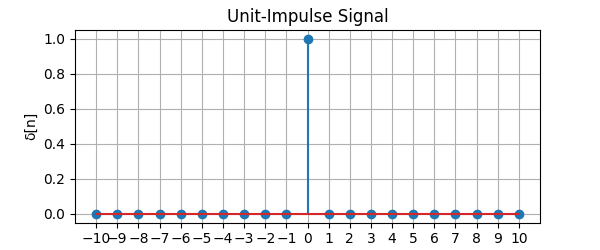
\includegraphics[scale=0.925]{./Assets/solution-1a-1.png}
            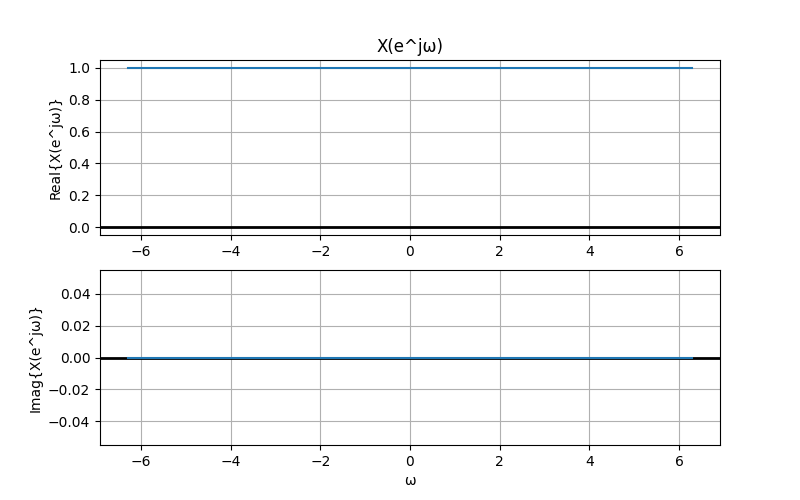
\includegraphics[scale=0.7]{./Assets/solution-1a-2.png}
            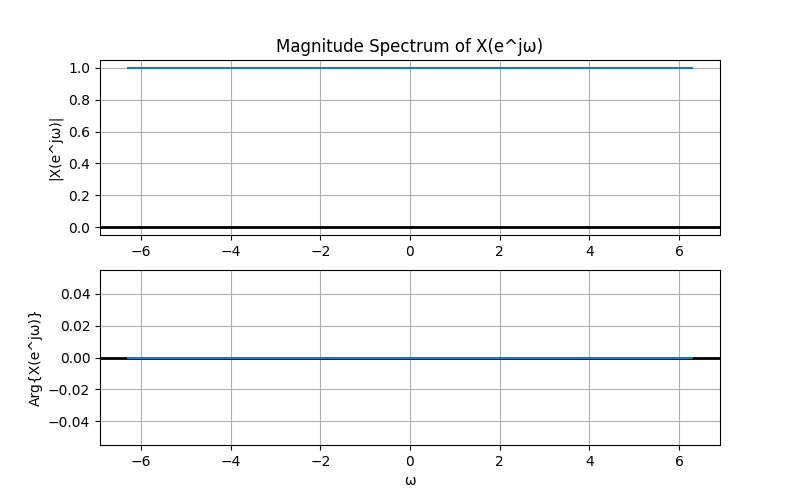
\includegraphics[scale=0.7]{./Assets/solution-1a-3.png}
            \caption*{Subplots for \textbf{Question: 1 (a)}}
        \end{figure}

        \pagebreak

        \begin{figure}[ht]
            \centering
            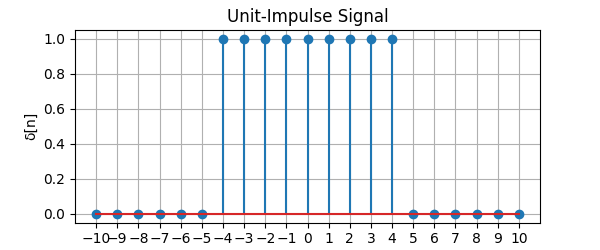
\includegraphics[scale=0.925]{./Assets/solution-1b-1.png}
            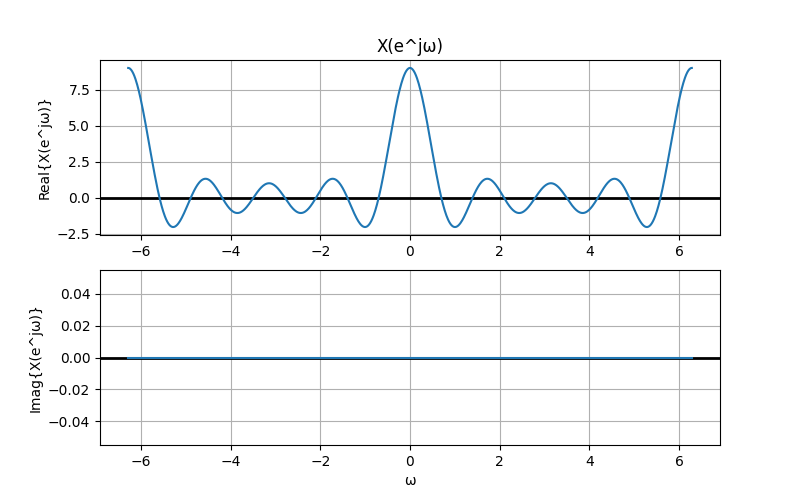
\includegraphics[scale=0.7]{./Assets/solution-1b-2.png}
            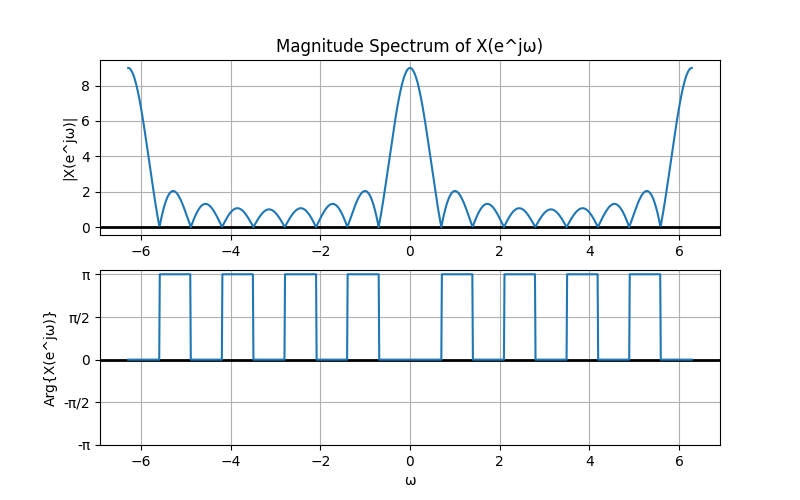
\includegraphics[scale=0.7]{./Assets/solution-1b-3.png}
            \caption*{Subplots for \textbf{Question: 1 (b)}}
        \end{figure}

    \end{enumerate}

\end{document}